\chapter{Návrh}\label{text:navrh}

\begin{chapterabstract}
Tato kapitola představuje návrh architektury aplikace s důrazem na její modularitu, škálovatelnost a udržitelnost. 
Zabývá se rozvržením klientské a serverové části, volbou technologií a organizací kódu. 
Dále rozebírá klíčové prvky systému, jako je editor a přehrávač materiálů, možnosti komunitního rozšíření pomocí pluginů a bezpečnostní mechanismy pro ochranu uživatelských dat. 
Kapitola nabízí hlubší pohled na rozhodnutí, která ovlivní aktuální, ale i budoucí vývoj platformy.
\end{chapterabstract}

\section{Architektura}

Návrh architektury je klíčový~\cite{uml_2007} pro správný softwarový vývoj. 
Jeho cílem je vytvořit aplikaci a kód tak, aby byly snadno rozšiřitelné, přehledné a jednoduché k údržbě. 
Pokud je architektura špatně navržena~\cite{uml_2007}, programátoři na ni často navazují a problémy se dále prohlubují.
Kód bývá často psán ve spěchu bez ohledu na budoucnost. 
Funkcionality lze implementovat různými způsoby, avšak důležité je myslet na možnost budoucího rozšíření~\cite{sutherland_2014} a refaktorizace. 
Nepřehledný kód znesnadňuje jeho úpravy, údržbu i rozšiřování.

Základním~\cite{richards_2020} prvkem architektury je definování odpovědností jednotlivých částí systému. 
Vzhledem k požadavku na webovou aplikaci byl zvolen model klient-server. 
Tento model je široce využíván~\cite{richards_2020, uzayr2022frontend}, jelikož umožňuje vývoj multiplatformních aplikací, které lze používat na různých zařízeních. 
Klient může být vyvíjen nezávisle na serveru, přičemž je klíčové jasně definovat rozhraní pro vzájemnou komunikaci. 
V této aplikaci se bude ke komunikaci používat zabezpečený protokol HTTPS.

Klientská část zpravidla představuje uživatelské prostředí běžící na zařízení uživatele a závisí na serveru. 
Serverová část zpracovává požadavky, odpovídá na ně a komunikuje s databází, externími službami nebo zajišťuje odesílání e-mailových zpráv. 
Hlavní stránka slouží k reprezentaci projektu.
Následující části textu se věnují podrobnostem o struktuře jednotlivých komponent, použitých technologiích a způsobu jejich rozdělení. 
Diagram návrhu architektury je vyobrazen na obrázku~\ref{fig:architektura}.

\begin{figure}[ht!]
    \centering
    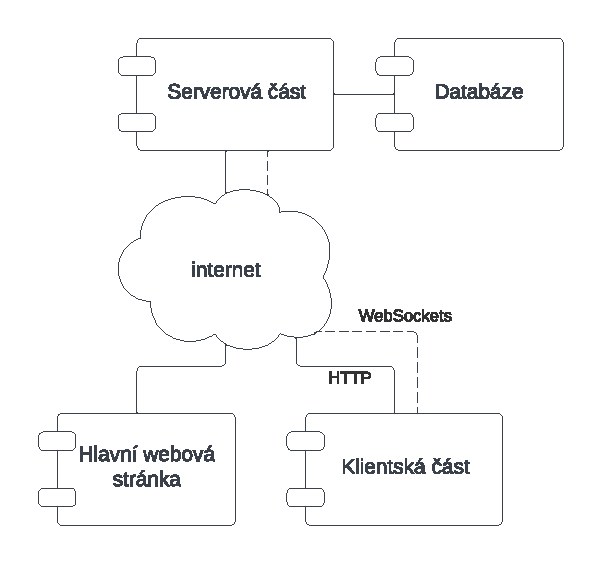
\includegraphics[width=1\textwidth]{media/04_navrh/architektura.pdf}
    \caption{Diagram architektury aplikace}\label{fig:architektura}
\end{figure}
 
\subsection{Klient}\label{text:navrh/klient}

Klientem celé aplikace bude webová stránka, ve které budou uživatelé vytvářet, přehrávat a procházet materiály. 
Obecně na této části budou uživatelé ovládat celou aplikaci.
Webová stránka je vhodná, protože to dovolí rychlejší přístup ke všem funkcionalitám bez nutnosti cokoliv instalovat.
Instalace taktéž není vhodná kvůli velkému počtu používání materiálů studenty, kterým by toto stahování mohlo přijít nevhodné.
Později by šlo z aplikace vytvořit nativní aplikaci na desktop či telefony pomocí enkapsulace webové stránky.
Dále je vhodné vyřešit, jestli aplikace bude \enquote{single page application} či \enquote{multi page application}.
Použiji SPA oproti alternativě a to z důvodu, že obnovení stránky není na takto velké aplikaci vhodné.
Hlavním cílem stránky je editor, což je zcela klientská komponenta, která by při alternativě nebyla dobře stvořitelná.  

Tato část bude pomocí REST API komunikovat se serverovou částí za pomoci protokolu HTTP, ze které bude získávat veškerá potřebná data.
RESTful API je ve zkratce takové API, které pracuje se zdroji jako takovými a dovoluje nad nimi volat klasické akce jako čtení, přidání, smazání a změnu (CRUD).
Mimo jiné definuje další standardizované chování, které by toto API mělo mít.
Tento způsob dovoluje tvořit tzv. \enquote{thick klienty}, které vysvětlím a zdůvodním později.

Klient tedy poběží ve webovém prohlížeči uživatele.
Díky tomu tedy musí být klient definován a stylován za pomocí HTML a CSS.
Kontrola samotné stránky musí být ve skriptovacím jazyce JavaScript.
Pro bezpečnější a udržitelnější~\cite{typescript_docs} kód však v této aplikaci použiji typovanou nástavbu TypeScript, která se kompiluje do čistého JavaScriptu.
Klient bude tvořen v myšlence \enquote{thick klienta}~\cite{uzayr2022frontend}, tedy většinu funkcionalit by měl implementovat klient za pomoci dat a služeb, které dostane (má k dispozici) od serveru.
Toto dovoluje odlehčit server náročnými požadavky (překreslením HTML na serveru při každé akci a podobně) a soustředit se pouze na to důležité.
Klient taktéž bude moci být používán s menší závislostí na serveru a při správném nastavení například i dále dovolovat čtení, i když uživatel nebude připojen k internetové síti.
Nevýhodou je zátěž a dostupné funkcionality na zařízení, na kterém webová stránka poběží, ale to by na dnešních zařízeních neměl být žádný problém.

V sekci~\ref{text:vykreslovani} zmiňuji různé způsoby vykreslování obsahu na webových stránkách.
I když je analýza směřována zejména na obsah, tak podobné myšlenky, zejména z sekce~\ref{text:vykreslovani/html} lze aplikovat i na zbytek webových stránek.
Zjednodušeně, tvoření komplexních webových aplikací s mnohými funkcionalitami (což v tomto návrhu pro aplikaci plánuji) nelze dělat udržitelně pouze se základními funkcionalitami HTML, CSS a JS.
Pro komplexní \enquote{thick klient} webovou aplikaci je nutné~\cite{uzayr2022frontend} v moderním světě webového vývoje použít framework, který za nás bude řešit nejen uvedené:

\begin{itemize}
    \item Správu stavů aplikace a synchronizaci dat mezi komponentami.
    \item Efektivní aktualizaci a vykreslování uživatelského rozhraní.
    \item Modularizaci kódu pro lepší přehlednost a údržbu.
    \item Optimalizaci výkonu při práci s DOM (například virtualizaci seznamů).
    \item Zajištění kompatibility s různými zařízeními a prohlížeči.
    \item Možnost snadného rozšíření o další funkcionality pomocí dostupných knihoven a ekosystémů.
    \item Automatizaci testování a zajištění stability kódu.
    % \item Podporu pro server-side rendering (SSR) nebo static site generation (SSG), pokud je to potřeba.
\end{itemize}

Jako webový framework pro klient použiji knihovnu Vue, která je známá~\cite{potter_2023} pro svoji jednoduchost, stabilitu a komunitu.
Dobrou alternativou by byl například React, který byl vytvořen pro podporu velkých a komplexních aplikací, avšak s ním nemám tak velké zkušenosti.
Z výběru jiného frameworku nedostanu žádné benefity na více, a tedy preferuji použití něčeho, v čem mám největší zkušenosti.
Vue podporuje programování za pomocí TypeScript a taky typovanou nástavbu použiji.

\subsubsection{Vrstvy a zodpovědnosti}

Klientská (a i serverová) část bude dále rozdělena na další části (tzv. vrstvy) pro zjednodušení celého systému zodpovědností v aplikaci.
To povede k přehlednějšímu kódu a jednodušším změnám v celé aplikaci.
V realizované aplikaci budou vrstvy pak dále děleny a bude vytvořena další abstrakce.
Níže jsou naplánované veškeré vrstvy pro klientskou část.

\begin{description}
    \item[Komponenty] které zajišťují unifikované chování pro často opakující se prvky na stránce tak, aby jejich tvorba byla co nejrychlejší a dovolovala přehlednější kód. Komunikují se stránkami pomocí dvoucestných vazeb či událostí.
    \item[Stránky] které seskupují komponenty a vlastní funkcionality do jednotlivých stránek aplikace. Předávají komponentám data a určují jim, jak se mají chovat či zobrazovat.
    \item[Perzistence] které jsou často nazývané ve webovém inženýrství jako obchody (stores), které globálně ukládají data pro celou aplikaci, aby bylo jedno místo (či místa), kde je lze najít. Slouží k tomu, aby se o data nežádalo více, než je nutné (caching). Mohou dovolovat ukládat data zcela perzistentně i mezi načtením stránky pro rychlejší prvotní načtení. Komunikují se serverem pomocí další vrstvy.
    \item[Komunikace] zajišťuje komunikaci se serverem pomocí RESTful API serveru. Určují a kontrolují jaká data od serveru přijdou, určují lokální rozhraní pro CRUD operace s danými zdroji a mapují je na lokální objekty.
\end{description}

\subsubsection{Editor a přehrávač}

Nejklíčovější částí klienta je editor a přehrávač materiálů, které budou uživatelé tvořit.
Editor i přehrávač jsou příliš komplexní a vzhledem k cíli práce vytvořit jednoduše rozšiřitelnou aplikaci (a to i díky komunitnímu rozšíření) proto není vhodné pro tyto části webové aplikace použít zmíněný framework.
Rozšiřování frameworku by bylo velmi zvláštní a nebylo by to příliš intuitivní.
Hlavním problémem je však ztracení jakékoliv kontroly, jak a kdy se vykresluje daný obsah, který framework spravuje.
Z tohoto důvodu musí být takto komplexní komponenta, tedy editor a přehrávač, manuálně spravována.
Naštěstí framework Vue dovoluje označit část kódu jako spravovanou někým jiným a tento prvek nebude překreslovat, pokud se nezmění jeho závislost (tedy pokud mu to kód neoznámí). 
Takovéto fundamentální rozdělení taktéž dovolí, že editor se může velmi jednoduše přidat i do jiných projektů či komponent.

V pozdější sekci~\ref{text:navrh/editor_player} je rozepsáno, jak hodlám řešit to, jak se bude obsah zobrazovat v editoru a přehrávači, jak se bude upravovat, definovat a podobně.

\subsection{Server}\label{text:navrh/server}

Cílem serverové části je poskytovat data klientské části a to kvůli \enquote{thick klientu}. 
Tato data bude server získávat z dalších služeb a zejména z databáze, ve které budou data perzistentně uložena.
O databázi se budu dále rozepisovat v sekci~\ref{text:navrh/databaze}.
Mezi další služby bude patřit e-mailový server či různá další externí API třetích služeb (například na získávání obrázků z datových bank a tak dále).

Poskytované API, což jsem zmínil v sekci~\ref{text:navrh/klient}, bude RESTful a tedy bude dovolovat práci se zdroji. 
Alternativní způsob designu API~\cite{richardson_2013} je například Simple Object Access Protocol (SOAP), který dovoluje volání akcí na serveru.
Standard REST API, jakožto moderní způsob komunikace, ukládá za povinnost takové věci API, které se slučují s navrhovanou aplikací.
SOAP by byl v tomto případě nevhodný a to zejména z důvodu, že server v tomto případě zejména slouží jakožto služba, která ukládá data.
Většina funkcionality v celém projektu je na klientské části, ve které se materiály vytváří a prezentují.

Server bude získávat vstupní data z URL adresy, těla a hlavičky požadavku.
Požadavky i odpovědi na a ze serveru budou komunikovat zejména v JavaScript Object Notation (JSON).
JSON~\cite{richardson_2013, uzayr2022frontend} je jednoduchý formát, který se jednoduše implementuje skoro v každém jazyce a je postaven na bázi seznamu klíčů a příslušných hodnot.
Hodnoty mají mnoho podporovaných datových typů.
Server by měl být však připraven na jakýkoliv formát dat.
Mělo by být možné velmi jednoduše změnit například na formát Extensible Markup Language (XML).

Serverová i klientská část by měly sdílet společné rozhraní definující vstupní a výstupní formát dat aplikace.
Těmto objektům se říká Data Transfer Object (DTO).
Tyto objekty dovolují jednoduše typovat data, která vstupují a vystupují z REST API.

Některé koncové body a zdroje API musí být zabezpečené pomocí autorizace a autentizace. 
O zabezpečení budu mluvit v pozdější sekci~\ref{text:navrh/auth}.
Některé koncové body musí být limitované i pomocí \verb|rate-limiter|, tedy že omezí počet volání daného koncového bodu pro konkrétního uživatele či globálně.
Jedná se např. o stránku s registrací.

Samotná serverová část bude tvořena v jazyce TypeScript.
Volba TS je stejná jako v klientské části (viz sekce~\ref{text:navrh/klient}) a to tedy, že nutí programátora psát udržitelný kód, který je staticky typově zajištěn.

Implementace komunikačního uzlu je možná přes řadu způsobů a knihoven.
V JS, resp. TS ekosystému patří mezi nejoblíbenější~\cite{brown2019web} backendový rámec knihovna Express.js (často taktéž Express).
Express je knihovna k vytvoření HTTP serveru, která dosahuje velmi úctyhodných rychlostí odpovědi a je velmi jednoduchá na pochopení.
Alternativní jako nejoblíbenější bývá~\cite{poreba_2023} zmiňována knihovna Fastify.
Právě Express jsem se rozhodl použít díky své malé velikosti, komunitě a jeho velké stopě v ekosystému.
Express má řadu předpřipravených funkcionalit jako jsou routery, middleware a mnoho dalšího.

I přes to, že má Express mnoho připraveného, jeho používání bez jakékoliv nástavby je vhodné jen pro projekty, kde jde zejména o rychlost, a to i rychlost vývoje.
Pro udržitelnější servery je vhodné použít nějaký framework, který staví nad těmito knihovnami a dovoluje rychlejší zápis kontrolérů, modulů a služeb s pomocí Dependency Injection (DI).

Mezi nejznámější frameworky~\cite{uzayr2022frontend, nest} v JS ekosystému, které používají (nebo dovolují) Express, patří například NestJS či Koa.
Mezi nejvíce~\cite{nest} oblíbené patří však NestJS a to zejména díky své velké komunitě, dokumentaci a rychlosti.
NestJS řeší vše dříve uvedené a mnoho dalšího.
Dovoluje rapidně tvořit udržitelné webové servery s HTTP API a podporuje řadu způsobů a knihoven návrhu.
Jedná se např. o passport, Mongo, Prisma, fronty úkolů, volání úloh, CORS, verzování API a mnoho dalšího.
Proto jsem se rozhodl NestJS s Express použít a to za pomoci TypeScriptu.

Server nejspíše bude používat i řadu dalších knihoven, například na odesílání e-mailů, jejich formátování a například na generování přihlašovacích tokenů pomocí JWT (viz sekce~\ref{text:navrh/auth}).
Tyto knihovny budu zajišťovat během vývoje aplikace.

V aplikaci plánuji vytvořit kolaboraci v editoru materiálu a další real-time komunikaci, a proto je potřeba zajistit tento mechanismus.
Možné je používat např. metody polling, long polling, server-sent events a další~\cite{subramanian_2021}, které běží přímo za pomoci protokolu HTTP.
Vhodnější je dle mého použít protokol WebSocket, který je přesně pro real-time oboustrannou komunikaci určen~\cite{rfc6455}.
Na serveru lze používat různé knihovny.
Mezi nejznámější~\cite{uzayr2022frontend} patří např. \verb|ws| či \verb|socket.io|.
Právě \verb|socket.io| jsem si vybral z důvodu, že umí například řešit nepřístupnost WS či umí rozdělovat uživatele do skupin, ve kterých se odděleně komunikuje.

Výsledné API, které vznikne z této aplikace, se pokusí dodržovat vše, co uvádí standard REST.
To souvisí i s návrhem jednotlivých koncových bodů, které budou řádně uvádět stavové kódy, dodržovat metody komunikace a řadu dalších.

\subsubsection{Vrstvy a zodpovědnosti}

I serverová část bude rozdělena do vrstev. 
Základ těchto vrstev je definován rovnou ve vybraném frameworku NestJS.
Avšak vrstev tam je definováno přespříliš, a proto hodlám používat jen část z nich.
V realizované aplikaci budou vrstvy pak dále děleny a bude vytvořena další abstrakce.
Níže jsou naplánované veškeré vrstvy pro serverovou část.

\begin{description}
    \item[Moduly] Ty sumarizují následující vrstvy do jednotlivých balíčků, se kterými se dá jednoduše pracovat. Definují co se má exportovat a importovat v rámci DI.
    \item[Služby] Ty sumarizují společné funkcionality do jednoho balíčku, aby se kód nemusel opakovat. Vztahují závislosti a agregují další služby a modely. Dají se sem počítat i tzv. Guardy, které kontrolují zda bude požadavek potvrzen a v aplikaci dále předáván do funkcí kontroleru.
    \item[Kontroléry] Ty tvoří REST API, volají funkce služeb, určují vstupní a výstupní data včetně návratových kódů.
    \item[Modely] Ty definují schéma databáze, respektive jednotlivých entit uvnitř.
\end{description}


\subsection{Databáze}\label{text:navrh/databaze}

Databázová část je zodpovědná za ukládání dat a poskytování rozhraní pro čtení a úpravu daných dat. 
V této části je potřeba databáze, respektive systém řízení báze dat (SŘBD).

Mezi zvažované možnosti jsem prvně přemýšlel o PostgreSQL a MongoDB.
Tyto dvě databáze poskytují základní spektrum pro databáze a to jsou~\cite{irena2015big, marek2018sql} SQL a NoSQL databáze. 
Aplikace jako celý cíl má stanovené to, že má být v budoucnu rozšiřitelná.
Je možné si představit, že tato aplikace bude v budoucnu ukládat velmi mnoho dat a bude potřeba, aby databázový stroj podporoval horizontální i vertikální škálování.
Podobně data, která budou v databázi uložena, nemají jasně stanovenou strukturu a obecně se bude jednat o velmi komplexní objekty.
V této aplikaci je lepší ztratit konzistenci dat, která např. MongoDB negarantuje (resp. je v módu \enquote{někdy bude konzistentní}~\cite{irena2015big}), důležitá je dostupnost a odolnost k přerušení.
I když budou na sebe data ukazovat (viz datový model v sekci~\ref{text:analyza/datovymodel}), jsou tato propojení velmi triviální a spíše je vhodné dokumenty do sebe vnořovat.
Proto nevidím důvod na použití relační databáze a to i kvůli struktuře dat.

Alternativou s podobnými vlastnostmi~\cite{irena2015big} jako MongoDB je CouchDB a Firebase Firestore. 
CouchDB je dokumentová databáze, která využívá JSON pro ukládání dat, podporuje replikaci a je navržena pro distribuované systémy. 
Její hlavní výhodou je tzv. \enquote{multi-master} replikace, která umožňuje synchronizaci mezi více instancemi databáze. 
Firestore, jako součást ekosystému Firebase~\cite{firebase}, nabízí jednoduché škálování a real-time synchronizaci, což je výhodné pro aplikace s požadavky na okamžitou aktualizaci dat mezi uživateli. 
Nicméně, Firestore je úzce spjat s Google Cloud platformou a může být nákladnější v závislosti na objemu provozu a požadavcích na škálovatelnost. 
Vzhledem k těmto faktorům jsem se rozhodl zvolit MongoDB, která poskytuje dostatečnou flexibilitu pro strukturu dat i škálovatelnost bez závislosti na konkrétním poskytovateli cloudových služeb.

Díky výběru knihovny Nest (viz sekce~\ref{text:navrh/server}) je vhodné pro databázi použít takový driver, aby s ním i daná knihovna uměla pracovat.
V základním rozpoložení umí Nest pracovat mimo jiné s drivery (resp. ODM/ORM) Mongoose a Prisma~\cite{nest_database}.
S Mongoose mám velmi velké zkušenosti a používám ho i v projektech mimo Nest.
Prisma je na druhou stranu velmi populární nejen pro MongoDB, ale i pro ostatní databázové stroje.
Prisma má však velké problémy s MongoDB -- například se jedná o pomalejší dotazování\footnote{např. issue: \url{https://github.com/prisma/prisma/issues/16916}} či často je nutné velmi složitě nastavovat server~\cite{prisma_2025}.
Definice entit a jejich závislostí je taktéž velmi omezená.
Proto jsem se rozhodl použít s MongoDB právě knihovnu ODM mongoose.

\subsection{Databázové schéma}

Přestože návrh využívá nerelační databázi MongoDB, která nevyžaduje pevné schéma, je struktura dat vynucena pomocí ODM Mongoose na serveru.
Konzistenci dat tedy zajišťuje samotná aplikace při jejich zápisu a čtení. 
Pro vytvoření databázového schématu bylo nutné vycházet z doménového modelu a provedené analýzy ze sekce~\ref{text:analyza/datovymodel}.

Navržené databázové schéma pracuje s relacemi, a proto jeho níže uvedená reprezentace není zcela přesná -- jde o hrubý návrh, kde jsou relace nahrazeny vazbami mezi jednotlivými dokumenty. 
V návrhu se rovněž nacházejí vlastnosti s datovými typy označenými otazníkem na konci, což signalizuje možnost absence dané hodnoty.
V kontextu MongoDB a JavaScriptu to znamená, že hodnota může být buď explicitně definovaná, nebo mít hodnotu \texttt{undefined}.

Entity v databázovém schématu odpovídají těm v doménovém modelu, avšak jejich názvy, atributy a další části byly přeloženy do angličtiny pro snadnější implementaci. 
Do návrhu byly doplněny další entity, dle provedeného návrhu aplikace, a také dekompozice vazeb typu \texttt{M:N}. 
% Schéma je uvedeno v diagramu v obrázku~\ref{fig:databazoveSchema}.

Kompletní definice realizovaných schémat jsou dostupné v kódové příloze ve složce \verb|/platform/server/| a jednotlivých modulech.
Jednotlivé entity jsou vždy označeny příponou \verb|.schema.ts|.
Každá entita obsahuje validaci, která definuje platné hodnoty, povinné atributy, unikátnost či požadovanou délku.

% \begin{figure}[ht!]
%     \centering
%     \includegraphics[width=1\textwidth]{chapters/navrh/databazoveSchema.pdf}
%     \caption{Diagram databázového schématu}\label{fig:databazoveSchema}
% \end{figure}

\section{Designový systém}

Uživatelské prostředí je klíčovou součástí~\cite{kholmatova_2017} každé aplikace, protože určuje, jak snadno a příjemně se v ní uživatelé budou schopni orientovat a pracovat. 
Je to nejen vizuální aspekt, ale i celková interakce mezi uživatelem a aplikací. 
Kvalitně navržené uživatelské prostředí~\cite{tidwell_2019} může zlepšit uživatelský zážitek a zvýšit efektivitu používání aplikace.

Při návrhu aplikace je dobré si dopředu rozhodnout, jak bude uživatelské prostředí vypadat, aby uživatelský zážitek z celé aplikace byl co nejlepší. 
To zahrnuje nejen grafickou podobu, ale i logické uspořádání jednotlivých prvků, navigaci a celkovou ergonomii rozhraní.

Uživatelské prostředí lze rozdělit do dvou částí~\cite{kholmatova_2017} -- samotný designový návrh a technickou implementaci. 
V podstatě se jedná o komplexní designový systém. 
Ten určuje, jaké komponenty aplikace obsahuje, jak vypadají, jaké mají parametry, ale hlavně jak spolu navzájem interagují. 
Jako komponenty si lze představit tlačítka, vstupní pole, záložky a další, ale i jejich stav, například zda jsou vypnuté, zda vypadají speciálně, jejich pozice a mnoho dalšího.

Mezi známé designové systémy~\cite{tidwell_2019, kholmatova_2017, uzayr2022frontend} patří například Material Design od společnosti Google, který se používá nejen v Google aplikacích a systémech. 
Dále se používají například Apple Human Interface Guidelines, které jsou určeny pro aplikace v ekosystému iOS a macOS, nebo Fluent Design System od Microsoftu, který se používá především v aplikacích pro Windows.

CSS frameworky jsou v podstatě knihovny předpřipravených stylů a komponent, které usnadňují tvorbu konzistentního designu. 
Mezi známé CSS frameworky patří Bootstrap, který je jedním z nejpopulárnějších frameworků díky své jednoduchosti a široké komunitě, Tailwind CSS, který umožňuje větší flexibilitu při stylingu, nebo Bulma, který je založen na flexboxu a poskytuje moderní a elegantní vzhled.

Designové systémy a CSS frameworky jsou velmi dobrým nástrojem, který ušetří zejména vývojářům čas s vymýšlením prvků a designu, ale i zejména s funkcionalitou jednotlivých komponent. 
Problémem bývá ale to, že upravovat design těchto komponent a celkovou interakci mezi nimi je skoro nemožné. 
Proto často dovolují pouze změnit základní styly a třeba barvy jednotlivých stavů. 
Stránky, které používají stejné designové systémy, často vypadají identicky, a například v případě Google (při dodržení všeho uvedeného) si spousta uživatelů může myslet, že daná aplikace je přímo od nich. 
Tyto systémy se často hodí na nástroje a aplikace pro dané platformy.
Pro odlišení mezi konkurencí je skoro nezbytné si vytvořit vlastní systém, design a přemýšlet nad tím, aby si uživatelé stránku zapamatovali. 
To souvisí s designovou identitou a všechny pojmy se tímto propojují.

Designové systémy často mají předpřipravené komponenty pro různá prostředí. 
Například Material Design je implementován pro framework Vue (který jsem vybral v sekci~\ref{text:navrh/klient}) v různých knihovnách, mezi nejznámější patří například Vuetify či Quasar.

Výsledná aplikace je sice nástroj, ale reálně by měla být použita a být něco nového. 
Chtěl bych, aby aplikaci ihned kdokoliv poznal. 
Proto jsem se rozhodl nepoužívat žádný předpřipravený designový systém a vytvořit pro tuto aplikaci speciální, který bude plně odpovídat požadavkům a unikátně reflektovat její funkčnost a estetiku.

\subsection{Komponenty a styly}\label{text:navrh/desgin/komponenty}\label{text:navrh/design/komponenty}

Designový systém budu zakládat na komponentách a jejich interakcích.
Jednotlivým komponentám, ale i celé stránce, budu implementovat design.

Ve své bakalářské práci~\cite{cajthaml_bp}, ale i v jiných projektech, jsem implementoval řadu designových systémů.
Dle mého názoru je důležité si rozhodnout zejména o typech komponent, které se budou využívat.

Níže jsou uvedeny komponenty, které bude zajisté nutné ve výsledné práci používat, a jejich krátký popis.
Celým seznamem se inspiruji zejména z již existujících projektů.
Plánuji taktéž použít část kódu z již vytvořených komponent, které jsem vytvořil.
Nějaké i z bakalářské práce, kterou jsem dále upravoval dle potřeb evoluce daného studijního informačního portálu. 

\begin{description} 
    \item[Upozornění] Slouží k upozornění uživatele na nějaký speciální stav – například chybu či varování. 
    \item[Tlačítko] K interakci s částmi aplikace, umožňuje akce, přesměrování a vizualizaci. 
    \item[Rozdělovač] Odděluje obsahové sekce pro lepší přehlednost. 
    \item[Dialog] Zobrazí modální okno pro potvrzení, zadání nebo informaci. 
    \item[Karta] Umožňuje organizaci obsahu do vizuálně oddělených bloků. 
    \item[Seznam] Strukturované zobrazení prvků pro snadnou orientaci. 
    \item[Záložky] Přepínání mezi různými sekcemi bez změny stránky. 
    \item[Stránkování] Rozděluje obsah na více stran pro lepší navigaci. 
    \item[Navigace] Umožňuje pohyb mezi různými částmi aplikace. 
    \item[Formulář] Sběr a odesílání dat od uživatele. 
    \item[Vstupní pole] Umožňuje zadání textových nebo číselných hodnot. Taktéž výběr z možností.
\end{description}

Mezi další základní styly, které bude nutné implementovat, patří:

\begin{itemize}
    \item Typografie a různé zvýrazňovací prvky.
    \item Grid systém pro rozdělení stránky do jednotlivých sloupců.
    \item Pomocné třídy na odsazení a základní rozložení, jako je například flexbox.
\end{itemize}

Komponenty se budou implementovat graficky, díky omezení a požadavkům na webovou stránku, pomocí HTML a CSS.
Funkčnost budu tvořit za pomoci interaktivního frameworku Vue.

Pro jednoduché grafické úpravy barev, odsazení a celkovou konzistenci skrz celou aplikaci je nutné implementovat tyto hodnoty jako proměnné.
Je možné je definovat jako nativní CSS proměnné či v nějakém CSS preprocesoru, jako je například Syntactically awesome style sheets (Sass).
Obě možnosti by byly dobrým rozhodnutím pro budoucnost projektu a ze dřívějších zkušeností však musím pro proměnné použít nativní CSS proměnné.
Ty jednodušeji dovolují měnit hodnoty za běhu a zároveň i dědičnost mezi prvky, což vytvoří systém, který reaguje na požadavky aplikace.
To taktéž dovolí vytvořit systém motivů, který bude měnit jednotlivé barvy v proměnných do předpřipravených stylů, které bude moci uživatel vybírat.

Přesto hodlám metajazyk Sass v práci používat, protože dovoluje například jednodušší vnořování jednotlivých selektorů či prosté cykly pro tvoření komplexních názvů pro pomocné třídy.
Sass je nutné kompilovat, naštěstí to řeší rovnou spojení Vite společně s Vue za pomocí knihovny \texttt{sass}.

Styly budu psát přímo ke komponentám a pomocné třídy do globálních souborů, které budou vždy načteny.

Responzivitu komponent budu řešit jednotlivě a všechny pomocné třídy budou mít podpůrné třídy nebo automaticky nastavenou responzivitu.
Responzivita bude fungovat na tzv. breakpoint mechanice (či zlomové body).
To zajišťuje, že stránka je responzivní vždy do určité šířky zařízení.
Na webové stránce těchto zlomových bodů bude několik, což dovoluje přizpůsobení na většinu zařízení.
Na obrovských (širokoúhlých) monitorech se stránka umístí doprostřed obrazovky a více se neadaptuje.
Stránka bude responzivní na výšku automaticky díky nepoužívání relativních jednotek vůči výšce.

\subsection{Návrhové obrazovky}

Wireframy (také označované jako návrhové obrazovky) slouží k rychlému náhledu uspořádání prvků a obsahu v připravované aplikaci. 
Oproti detailnějším prototypům či mockupům se u nich klade důraz především na pozici a význam prvků, nikoliv na finální grafické zpracování či prokliky mezi obrazovkami.

Vytváření návrhů pro tuto aplikaci probíhalo v nástroji Figma. 

Během práce jsem se inspiroval zejména svými již dříve vytvořenými uživatelskými prostředími a obecně z nástrojů, které jsem analyzoval v sekcích~\ref{text:analyza/prezentace},~\ref{text:analyza/grafika} a~\ref{text:analyza/materialy}.

Během práce bylo možné ihned provádět úpravy na základě zpětné vazby od uživatelů a lépe tak vyladit přehlednost nebo ergonomii rozložení. 
Více o testování a zpětné vazbě při tvorbě aplikace je k dispozici v kapitole~\ref{text:testovani}.
Každá z vytvořených obrazovek proto odráží aktuální požadavky na funkčnost i strukturu aplikace.


Celkem vzniklo 22 návrhových obrazovek, jejichž ukázky jsou uvedeny v obrázcích~\ref{fig:navrhovaObrazovkaRozsireni} a~\ref{fig:navrhovaObrazovkaEmailAKod}, zatímco úplný přehled všech návrhů lze nalézt v příloze~\ref{appendix:navrhoveObrazovky}.
Mezi ně patří:

\begin{itemize}
    \item Přihlášení, vytvoření účtu.
    \item Hlavní stránka, vytvoření, import materiálu.
    \item Editor, nastavení, rozšíření, práce s bloky.
    \item Přehrávač, malování.
\end{itemize}

Další stránky a rozložení budou tvořeny z těchto základních návrhových obrazovek.
Hlavní stránka aplikace bude tvořena v podobném designu, ale rozložením se bude podobat úvodním stránkám jiných produktů.

\begin{figure}[ht!]
    \centering
    \includegraphics[width=0.95\textwidth,page=21]{media/04_navrh/navhoveObrazovky.pdf}
    \caption{Návrhová obrazovka editoru s otevřeným vyskakovacím oknem s aktivními rozšířeními}\label{fig:navrhovaObrazovkaRozsireni}
\end{figure}

\begin{figure}[ht!]
    \centering
    \includegraphics[width=0.95\textwidth,page=12]{media/04_navrh/navhoveObrazovky.pdf}
    \caption{Návrhová obrazovka přihlašovací stránky v záložce \enquote{E-mail s potvrzením} po odeslání žádosti}\label{fig:navrhovaObrazovkaEmailAKod}
\end{figure}


\section{Návrh editoru a přehrávače}\label{text:navrh/editor_player}

Při návrhu platformy bylo nutné definovat základní komponenty systému, které umožní tvorbu, editaci a následné přehrávání interaktivních výukových materiálů. 
Klíčovými prvky jsou bloky jako nejmenší jednotky obsahu, editor sloužící k jejich úpravám a přehrávač, který umožňuje interakci s uživateli.

\subsection{Bloky}

Základním konstrukčním prvkem v navrhovaném systému je blok. 
Každý blok představuje samostatnou jednotku obsahu, která může nabývat různých podob. 
V rámci návrhu je definována sada základních bloků, které lze kombinovat a upravovat podle potřeb uživatele.

Základní typy bloků mimo jiné zahrnují:

\begin{description}
    \item[Textové bloky] Které dovolují formátování textu -- což zahrnuje změny velikosti, barvy, fontu a další.
    \item[Obrazové a multimediální bloky] Dovolují vkládání a různou manipulaci s obrázky, videi a dalším interaktivním obsahem
    \item[Tvarové bloky] Které umožňují vložit předdefinované tvary a jejich modifikaci.
    \item[HTML blok] Umožňuje skoro neomezeně rozšiřovat funkcionality prezentace pomocí psaní si vlastního HTML kódu, který se bezpečně vykreslí pomocí tagu Iframe.
\end{description}

Bloky mohou být mezi sebou uspořádávány, transformovány a jejich vlastnosti lze dynamicky měnit. 
Každý blok může obsahovat specifické vlastnosti, které ovlivňují jeho chování a vizuální reprezentaci.
Mezi základní vlastnosti patří pozice, velikost, průhlednost, otočení a řada dalších.
Dále je možné blokům nastavit různé stavy, které mohou sloužit jako vodítka pro editor při jejich správě, jako je například zamezení transformace a podobně.
To se hodí, pokud bloky mají existovat pouze v nějakém určitém místě.

\subsection{Editor}

Editor slouží jako prostředí, ve kterém jsou výukové materiály vytvářeny a poté upravovány. 
Uživatelé zde mohou vkládat a přemisťovat bloky, nastavovat jejich vlastnosti a provádět transformace všeho obsahu.

Hlavní funkce editoru zahrnují:
\begin{description}
    \item[Práce s plátnem] Což dovoluje nastavovat velikost plátna, se kterým bude uživatel pracovat, dovoluje přibližovat a hýbat s ním.
    \item[Práce s bloky] Dovoluje již zmíněné transformace, změny vlastností, interakce a dalšího.
    \item[Správa pluginů] Která dovolí upravovat nainstalované a aktivní pluginy, jejich aktualizace a používání. Každý plugin v editoru bude mít své připravené místo na jeho ovládání, viz sekce~\ref{text:navrh/plugins}.
    \item[Vkládání obsahu] Umožňuje vkládat obsah z veřejných knihoven (fotobanky a další), ale taktéž z uživatelských zdrojů, do kterých si uživatel může nahrát vlastní obsah.
    \item[Nastavení] Dovolí nastavit jméno, sdílení, viditelnost materiálů, způsob jeho průchodu a další.
    \item[Export] Dovolí uložit si kopie materiálu v různých formátech.
\end{description}

Editor informuje a reaguje na to, co dělá, například pomocí různých dialogů a vyskakovacích upozornění, aby umožnil intuitivní práci s materiály.

\subsection{Přehrávač}

Přehrávač je určen pro zobrazování a interakci s vytvořenými materiály. 
Uživatelé mohou obsah procházet, interagovat s prvky a využívat pokročilé možnosti zobrazení.

Funkce přehrávače zahrnují:

\begin{description}
    \item[Navigace] Přehrávač umožňuje procházet skrz snímky materiálu dle jeho nastavení. Tedy například průchod automaticky (časovačem), ručně či pouze pomocí interakce.
    \item[Pluginy] Dovolují upravovat a zobrazovat speciální obsah i mimo editor.
    \item[Interakce] Přehrávač dovoluje interagovat s prvky dle jejich nastavení.
    \item[Personalizace] Dovolují úpravu nastavení zobrazování podle preferencí uživatele.
\end{description}

Přehrávač je navržen tak, aby zajistil plynulou prezentaci obsahu a umožnil efektivní zapojení uživatelů do výukového procesu.

\subsection{Interakce v systému}

Interaktivita je klíčovou vlastností platformy.
Každý blok může obsahovat několik interaktivních nastavení, která reagují na různé akce. 

Mezi podporované interakce patří například časovače (po nějaké době, opakovaně) a různé uživatelské akce (kliknutí, najetí kurzoru) a mnoho dalšího. 

Po dané akci může interakce způsobit mnoho dalších akcí, například se jedná o:

\begin{itemize}
    \item Upravit vlastnosti sebe i cizích bloků.
    \item Změnit snímek.
    \item Resetování bloku či jeho vlastnosti.
    \item Změnu hodnoty proměnné. 
    \item Přesměrovat stránku na jinou URL.
\end{itemize}

Interakce se mohou spustit za nastavených určitých podmínek, jako je například čas na snímku, hodnoty proměnné a další.

Interakce jsou plně přizpůsobitelné a uživatelé mohou nastavit parametry, které určují jejich chování.
Lze taktéž nastavit animaci mezi jednotlivými stavy interakce.

\subsection{Architektura jádra}

Návrh tříd editoru a přehrávače tvoří základ celého systému. 
Promyšlená struktura těchto komponent je klíčová pro budoucí rozšiřování a udržovatelnost projektu.
Obrázek~\ref{fig:kodovyNavrhEditoruAPrehravace} ukazuje navržené jádro systému v hierarchii tříd.

Centrálním bodem architektury je třída \texttt{Editor}, která spravuje bloky typu \texttt{EditorBlock}. 
Tyto bloky pak mají jejich pozici, velikost a další vlastnosti jako neprůhlednost, uzamčení nebo například rotaci. 
Uživatel může s jednotlivými bloky manipulovat, přičemž každá změna je reflektována pomocí metod jako \texttt{move}, \texttt{rotate} nebo \texttt{resize}.
Kromě samotných bloků třída uchovává i informace o preferencích uživatele a selekci bloků prostřednictvím objektu \texttt{EditorSelector}.

Přehrávač (\texttt{Player}) má podobnou strukturu jako editor, ale využívá objekty typu \texttt{PlayerBlock}. 
Ty jsou zjednodušené a zaměřují se na vizualizaci a zpracování interaktivity. 
Zatímco editor slouží ke konfiguraci a návrhu, přehrávač reprezentuje výsledné zobrazení.
Bloky v editoru a v přehrávači mohou mít kompletně jiné funkcionality.

Důležitou součástí návrhu je třída \texttt{BlockRegistry}, která funguje jako registr všech dostupných bloků. 
Obsahuje záznamy (\texttt{BlockRegistryEntry}), jež propojují název bloku s jeho editační a přehrávací reprezentací a zároveň s deserializační logikou. 
Tato struktura umožňuje přehledně spravovat různé typy bloků bez závislosti na jejich konkrétní implementaci.

Serializace je řešena přímo v jednotlivých blocích.
Každý blok se umí převést do strukturovaného formátu, ve výsledné aplikaci se bude nejspíše jednat o JSON.
Opačný proces -- převod dat zpět do konkrétních instancí editorových či přehrávacích bloků -- zajišťuje třída \texttt{BlockDeserializer}, která je součástí každého záznamu registru.

Pro práci s více funkcemi v editoru je navržena třída \texttt{EditorSelector}. 
Toto je jedna z ukázkových tříd, které slouží na ukázání toho, že editor či přehrávač jsou tak velké komponenty, že je nutné je zmenšovat do samostatných modulů.
Mezi další moduly se bude řadit například schránka (clipboard) nebo kontextové menu. 

Je pravděpodobné, že výsledná implementace ještě zpřesní vztahy mezi jednotlivými třídami.
Například závislosti mezi \texttt{BlockRegistry}, \texttt{Editor} a \texttt{Player} mohou být v realizaci více oddělené nebo řešené přes kompozici.

\begin{figure}[ht!]
    \centering
    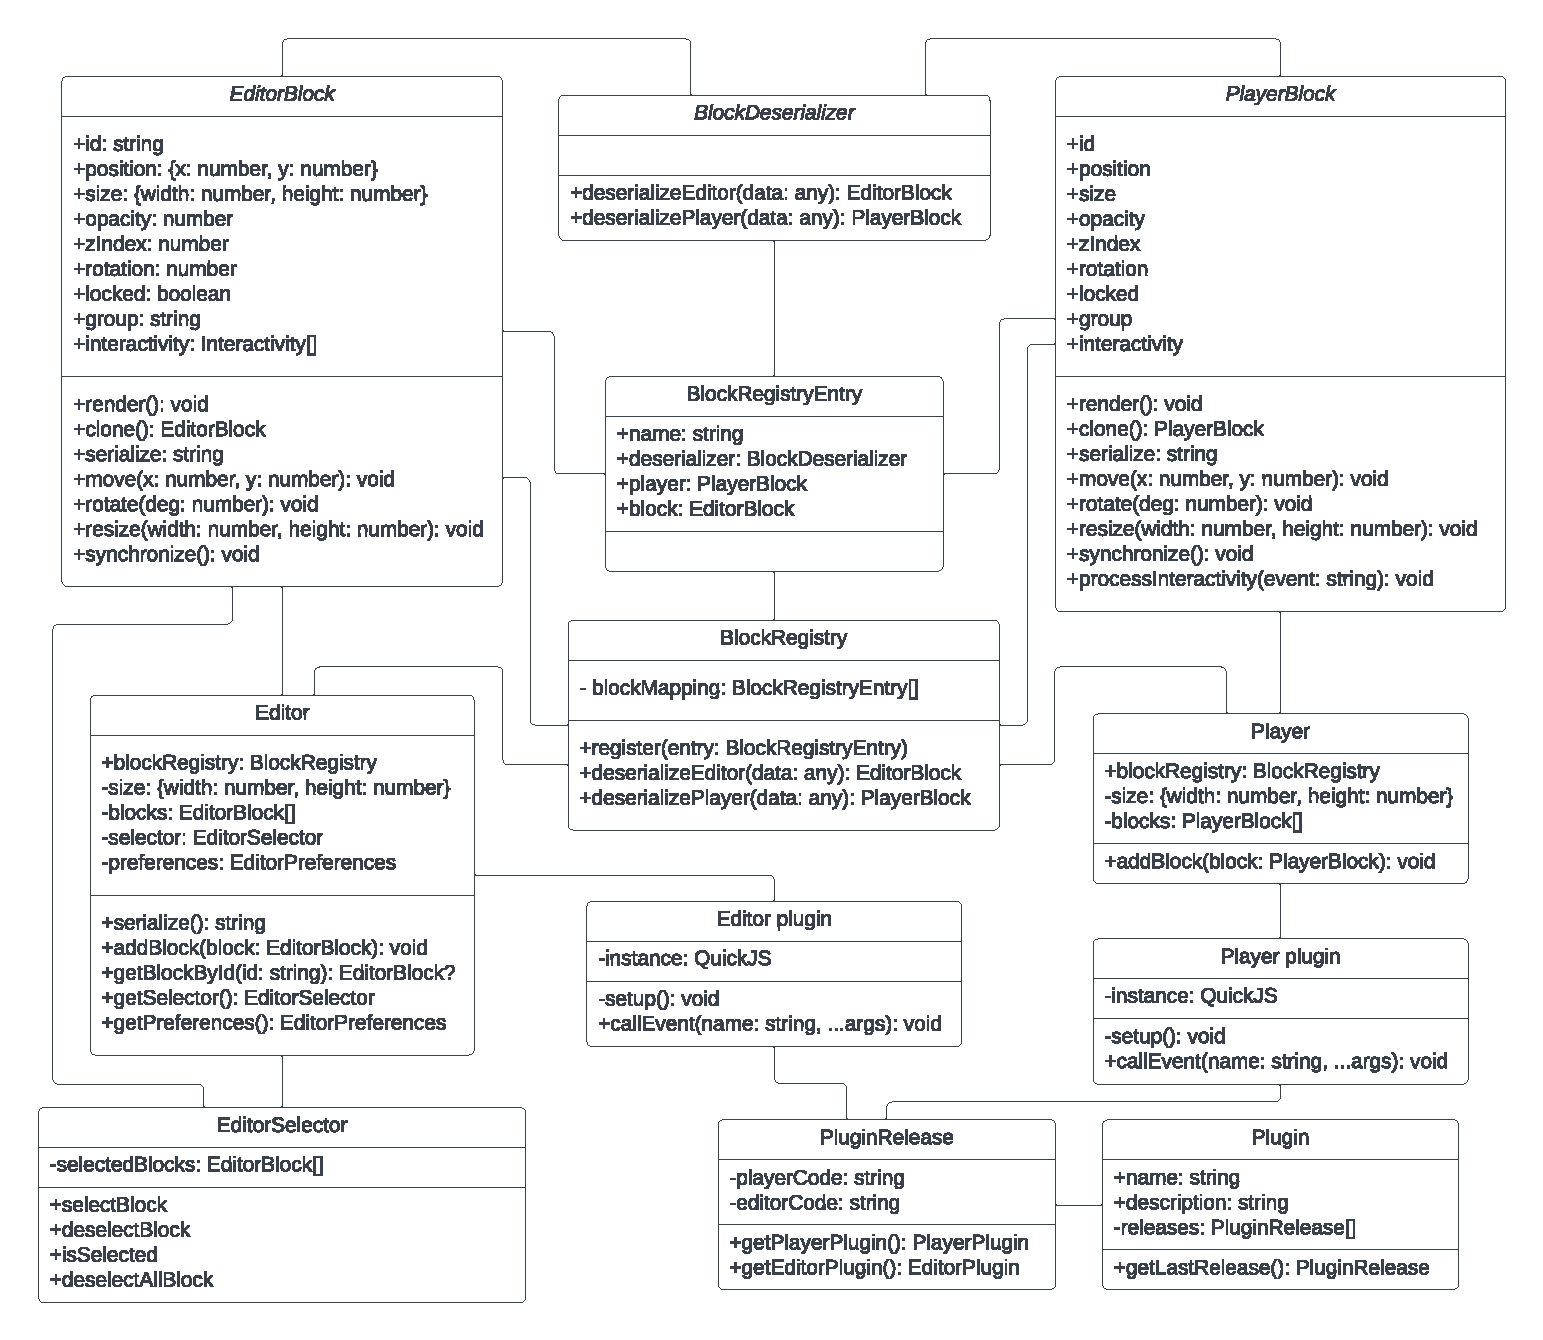
\includegraphics[width=1\textwidth]{media/04_navrh/kodovyNavrh.pdf}
    \caption{Kódový návrh editoru, přehrávače a připojených tříd}
    \label{fig:kodovyNavrhEditoruAPrehravace}
\end{figure}

\section{Návrh komunitního rozšíření}\label{text:navrh/plugins}

Navrhovaná platforma bude podporovat komunitní rozšíření, což umožní uživatelům přizpůsobit si prostředí dle vlastních potřeb a vytvářet nové funkce nad základním jádrem aplikace.
Klíčovými aspekty tohoto rozšíření jsou jazyková kompatibilita, bezpečnost, registrace API a způsob distribuce pluginů.
Základní analýzou tohoto byla sekce~\ref{text:community_plugins}.

Jako hlavní programovací jazyk pro komunitní rozšíření byl zvolen JavaScript.
Tento jazyk byl vybrán pro svou jednoduchost, širokou adopci a kompatibilitu s webovým prostředím.
Skripty budou spouštěny pomocí knihovny QuickJS, která umožňuje běh JavaScriptu na straně klienta s minimalizovanými bezpečnostními riziky díky využití WebAssembly.
Aby byla zajištěna integrace s editorem a přehrávačem platformy, bude vytvořeno API, které umožní pluginům komunikaci s těmito komponentami. 
Přímá abstrakce nad API nebude implementována, vzhledem k tomu, že zmenšení bezpečnosti QuickJS není pravděpodobné.
Pokud by se stala knihovna QuickJS nebezpečnou tak, že by z ní mohla jednotlivá rozšíření uniknout, budou pravděpodobně nefunkční všechna další jiná řešení.

Každý plugin bude sestávat z několika klíčových částí. 
Základem je manifest, který bude obsahovat základní informace o pluginu, jeho verzi a další nastavení. 
Další částí je samotný kód pluginu, který bude realizovat požadovanou funkcionalitu v přehrávači. 
Třetí část tvoří kód pro editaci v rámci editoru. 
V databázi platformy budou navíc uchovávána metadata, jako je název pluginu, jeho popis, informace o autorovi a jeho verze.

Systém verzování bude umožňovat udržení kompatibility s předchozími verzemi platformy. 
Nové verze pluginů budou vyžadovat aktualizovaný manifest, přičemž starší verze pluginů budou nadále funkční pro existující instalace. 
Uživatelé však nebudou moci instalovat starší verze pluginů, čímž se zajistí plynulá aktualizace celého ekosystému.
V rámci jedné instalace nebude možné mít aktivní více verzí jednoho pluginu současně.

Pro rozšíření funkcionality editoru i přehrávače bude možné registrovat API pro různé bloky a celý editor či plugin.
Editor bude umožňovat modifikaci velikosti, vytváření a úpravy jednotlivých bloků, zatímco přehrávač nabídne možnosti manipulace s přehrávaným obsahem, včetně navigace mezi snímky.
Mezi ostatními API budou různé debugovací nástroje, posílání požadavků či třeba systém cache pro ukládání dočasných dat.
Dále bude pro rozšíření možné registrovat panely přímo do uživatelského rozhraní, což umožní hlubší integraci pluginů.
Panely budou implementovány s využitím Iframe technologie, která zajistí izolaci kódu a zvýší bezpečnost systému.

Podobně bude vytvořen systém, kdy plugin bude moci vytvořit sám pro sebe určitý blok tak, že pouze on ho spravuje a vykresluje.
To dovoluje si ukládat speciální data a vytvořit řadu dalších funkcionalit.
Tyto bloky budou v podstatě již zmíněné HTML bloky, jen budou dovolovat ukládání dalších dat, registraci vlastních vlastností a další věci.

Rozšíření budou moci oběma směry komunikovat jak s pluginy, tak i s jednotlivými bloky.
To dovolí řadu budoucích rozšíření, kdy například kliknutí v panelu vytvoří blok, který může informovat plugin o tom, že se něco děje.

Bezpečnostní aspekty budou klíčovým prvkem návrhu.
Správné používání QuickJS je zásadní pro minimalizaci rizik spojených se spuštěním nedůvěryhodného kódu.
Komunikace mezi pluginy a hlavní aplikací bude co nejjednodušší, přičemž veškerá data budou podrobena validaci v každém použití.
Logování chyb a aktivit pluginů umožní lepší sledování a detekci potenciálních problémů.
Omezena bude také funkcionalita pluginů z hlediska síťové komunikace, zejména co se týče možnosti provádět HTTP požadavky (pomocí funkce \texttt{fetch}), čímž se zamezí neoprávněné komunikaci se servery třetích stran.
Uživatelé budou o speciálních povoleních pluginů obeznámeni před instalací.

Pro podporu komunitního rozšíření bude nutné zajistit i dokumentaci a nástroje, které usnadní vývoj pluginů. 
Dokumentace bude pokrývat jak základy tvorby pluginů, tak možnosti rozšíření kódu samotné platformy. 
Důraz bude kladen na snadnost implementace a přístupnost pro širší komunitu vývojářů.
Nejvíce klíčové bude, aby pluginy měly jasně vytvořený systém typování, který dovolí kontrolu pluginu před během a pomocí IDE dovolí uživatelům prozkoumávat celé API.

\section{Autentizace a autorizace}\label{text:navrh/auth}

Autentizace je proces ověřování identity uživatele, tedy zajištění, že se daná osoba skutečně nachází v systému. 
Typickými metodami autentizace jsou přihlašování pomocí uživatelského jména a hesla, biometrické údaje nebo autentizace prostřednictvím třetích stran.

Autorizace naopak určuje, jaká oprávnění má přihlášený uživatel v rámci systému.
Rozhoduje tedy o tom, ke kterým zdrojům má uživatel přístup a jak s nimi může nakládat.

\subsection{Autentizace}

V rámci této práce se autentizace soustředí na dvě základní metody přihlašování: kombinaci e-mailu a hesla a potvrzení pomocí odkazu zaslaného na e-mailovou adresu uživatele. 
Po úspěšné autentizaci se vygeneruje JWT (JSON Web Token), který slouží k ověřování uživatele během jeho aktivity v systému.

JWT token je podepsán na určitou dobu a obsahuje základní informace o uživateli, například jeho identifikátor a základní údaje pro rychlé vykreslení. 
Tento token se následně posílá v hlavičce požadavků \texttt{Authorization} pod typem \texttt{Bearer}, čímž je umožněno bezpečné ověřování uživatele při komunikaci se serverovou částí systému.

Uživatel si tento token ukládá lokálně, a to buď v cookies, nebo v local storage prohlížeče, což mu umožňuje zůstat přihlášený i po uzavření okna prohlížeče. 
Do budoucna je žádoucí rozšířit možnosti přihlašování například o autentizaci prostřednictvím OAuth, což by umožnilo přihlašování skrze služby třetích stran, jako je Google či Meta.
Aplikace na to musí být připravena.

\subsection{Autorizace}

Vzhledem k návrhu platformy není autorizace zatím příliš složitá. 
Hlavní princip spočívá v tom, že určité akce smí provádět pouze vlastník obsahu, což je validováno při každé operaci.
Například editace materiálu je povolena pouze jeho tvůrci. 

Dále jsou v systému prvky s nastavitelnou viditelností. 
Například materiál může být označen jako veřejný, což znamená, že si jej může prohlédnout kdokoliv. 
Podobně jsou některé části systému, například rozšíření (pluginy), standardně dostupné všem uživatelům.

V současné fázi vývoje platforma neobsahuje roli administrátora, což znamená, že neexistuje centrální správa uživatelů či jejich oprávnění. 
Toto rozhodnutí bylo učiněno s ohledem na jednoduchost návrhu, avšak do budoucna je možné uvažovat o zavedení administrativních funkcí pro efektivnější moderaci obsahu.
Dále budu diskutovat o administračním prostředí v kapitole~\ref{text:diskuze}.